
\chapter{The "XYZ" Prototype System}

% NOTES / TODOs:
%
% Architecture scheme, implementation
% callback functions, hot plugin
% js-select selectors
% List of condition operators
% Why JS, why wasnt it used before? is it used now?
% Transactions in businesses, find use case. how would we lose events?
% Terminierungsproblem (compiler bau), loesungsansaetze



\section{Event Triggers}

Event Gathering is the E in ECA and without one of these letters such a system would not run.
It is of utmost importance to find as much as possible ways to get data into a system.



\subsection{Polling for Events}



\subsection{Webhooks}
Which 



\section{Actions}



\section{ECA Rules}



\section{Architecture}



\section{Asynchronous Systems \& Closures}
% NOTES / TODOs:
%
% Variable bindings
% Closures (https://developer.mozilla.org/en-US/docs/Web/JavaScript/Guide/Closures)$
% Closures are functions that refer to independent (free) variables. 
% In other words, the function defined in the closure 'remembers' the environment in which it was created in.

% write about arallel as well?

Often optimization approaches and programming language concepts require special attention to avoid common pitfalls.
When closures are used in asynchronous systems, developers need to be very careful not to end up with randomly inconsistent states.


Looking at an example of sequential code execution in figure~\ref{fig:Closures_Synchronous}, we see that function execution of \texttt{fA} is halted until function \texttt{fB} is finished.
If \texttt{fB} happens to be a latency-driven I/O operation the completion of \texttt{fA} could be deferred for a relatively long time.
While the application waits for the completion of the I/O operation, some remaining operations in \texttt{fA} could eventually already be executed without causing any race conditions.
\begin{figure}[h!]
\centering
  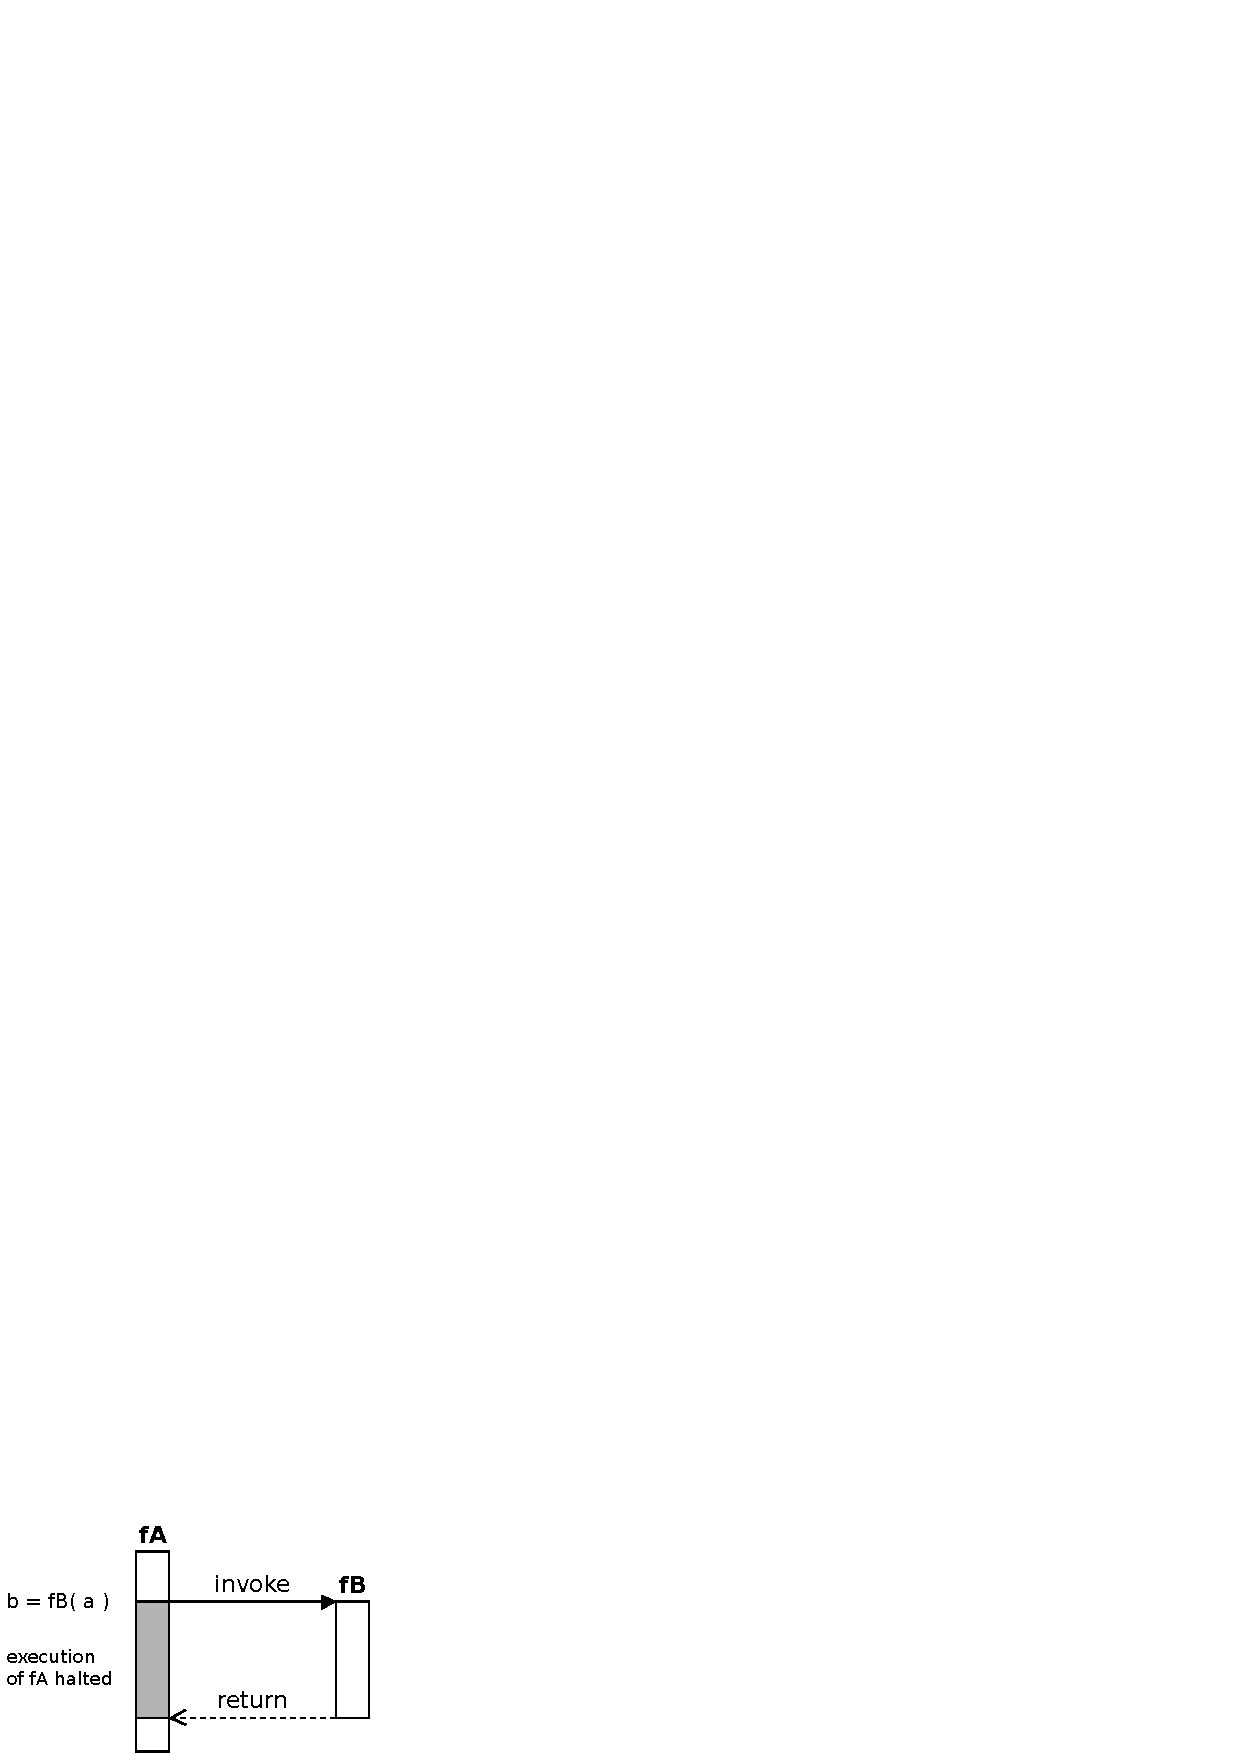
\includegraphics{figures/Closures_Synchronous}
\caption{Synchronous Function Call}
\label{fig:Closures_Synchronous}
\end{figure}


Asynchronous code execution, as shown in figure~\ref{fig:Closures_Asynchronous}, allows non-blocking and thus scalable applications.
Non-blocking operations are a remedy for optimzed resource allocation and open ways to overcome previously described unnecessary resource bindings.
Processing any kind of latency-driven I/O operation asynchronously ( e.g. filesystem access and socket communication ) exploits resources that would otherwise be bound while waiting for completion.
Such operations are processed and completed whenever required resources are available.
\begin{figure}[h!]
\centering
  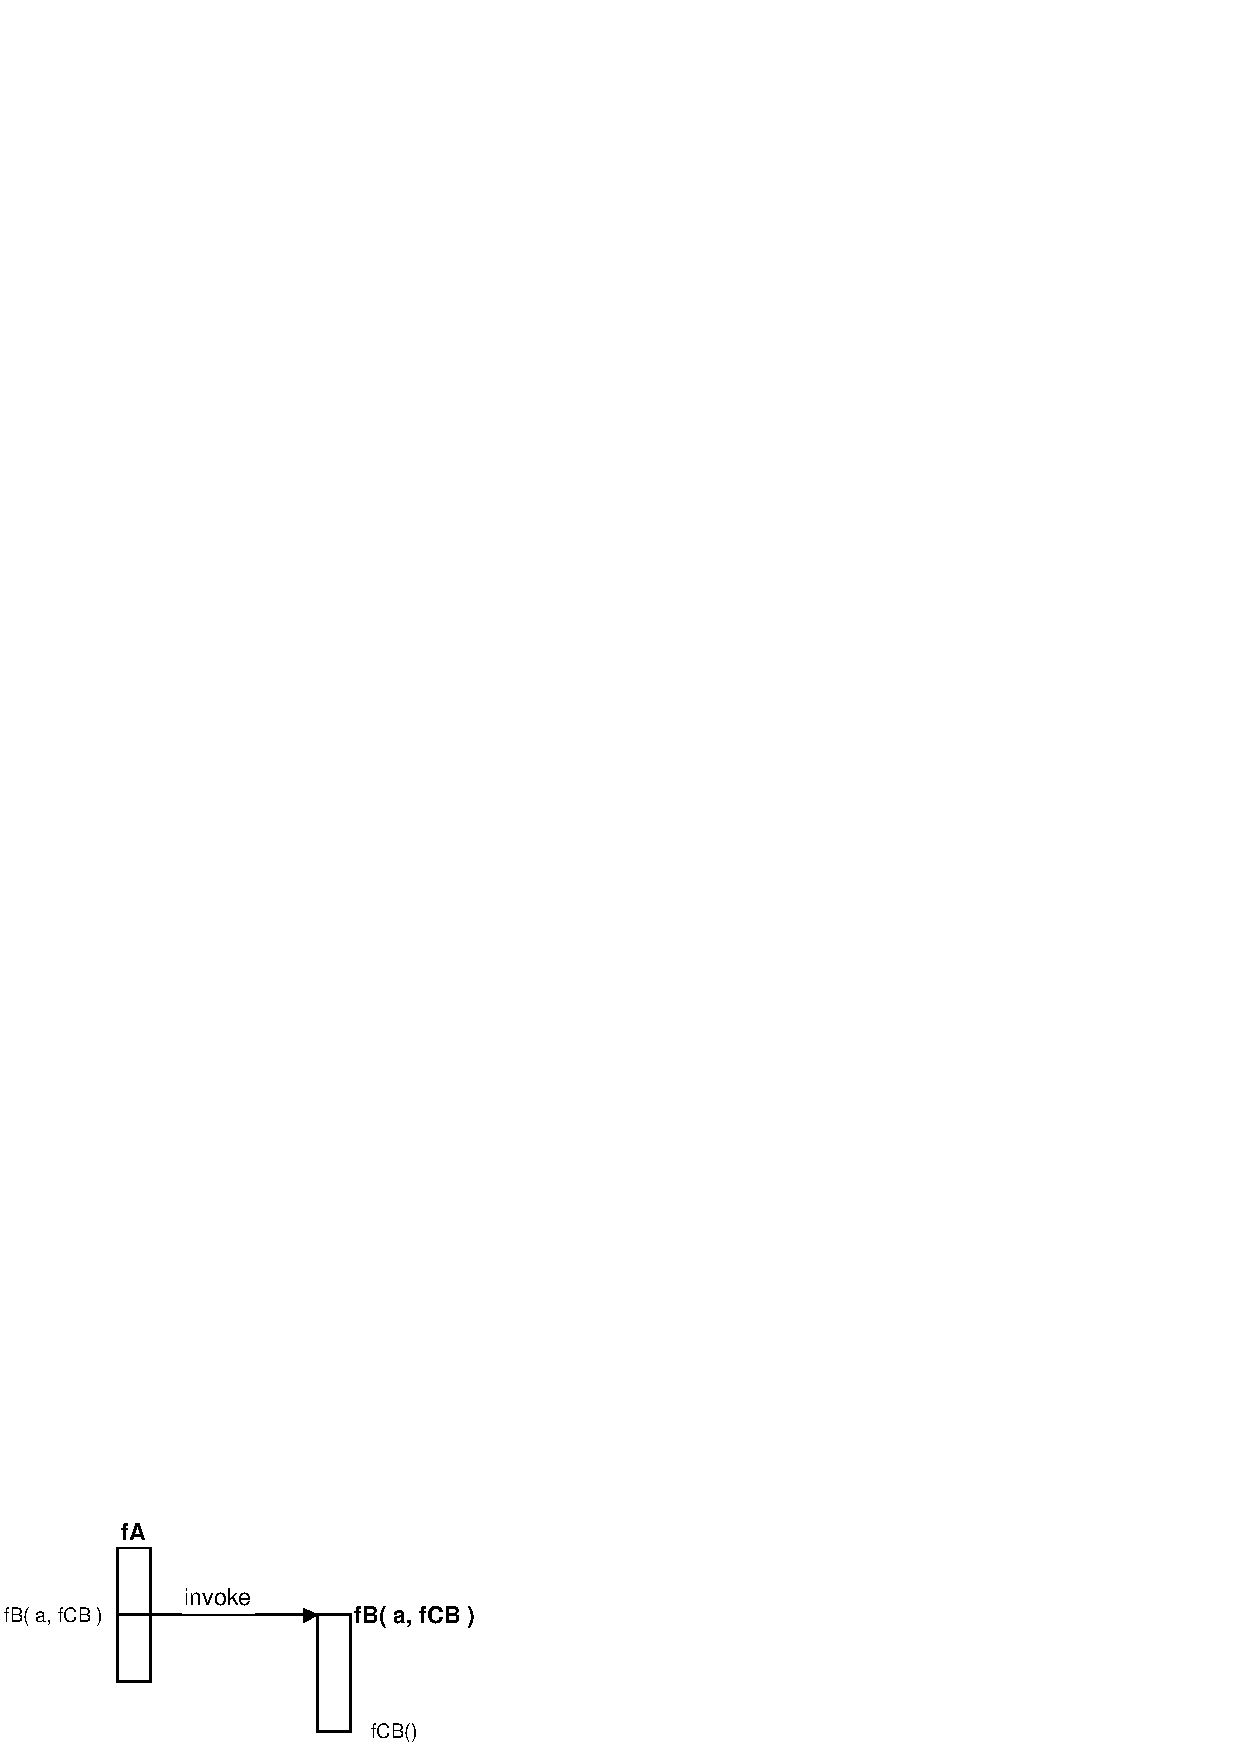
\includegraphics{figures/Closures_Asynchronous}
\caption{Asynchronous Function Call}
\label{fig:Closures_Asynchronous}
\end{figure}


Often other operations depend on the completion of asynchronous operations, hence their execution needs to be deferred.
This necessary code execution deferral is achieved through the use of callback functions, denoted \texttt{fCB} in figure~\ref{fig:Closures_Asynchronous}.
Any code placed in a callback function, which is assigned to an asynchronous operation, is only executed after the respective asynchronous operation completed.
This allows stacking of functions and operations upon each other which results in a flexible, event driven application.


If we look at the example in figure~\ref{fig:Closures_Asynchronous} and assume closures as defined in \cite{EcmaScript}, .
 


\begin{figure*}[htb]
%\begin{center}
\centering
%,angle=-90
  \makebox[\textwidth][c]{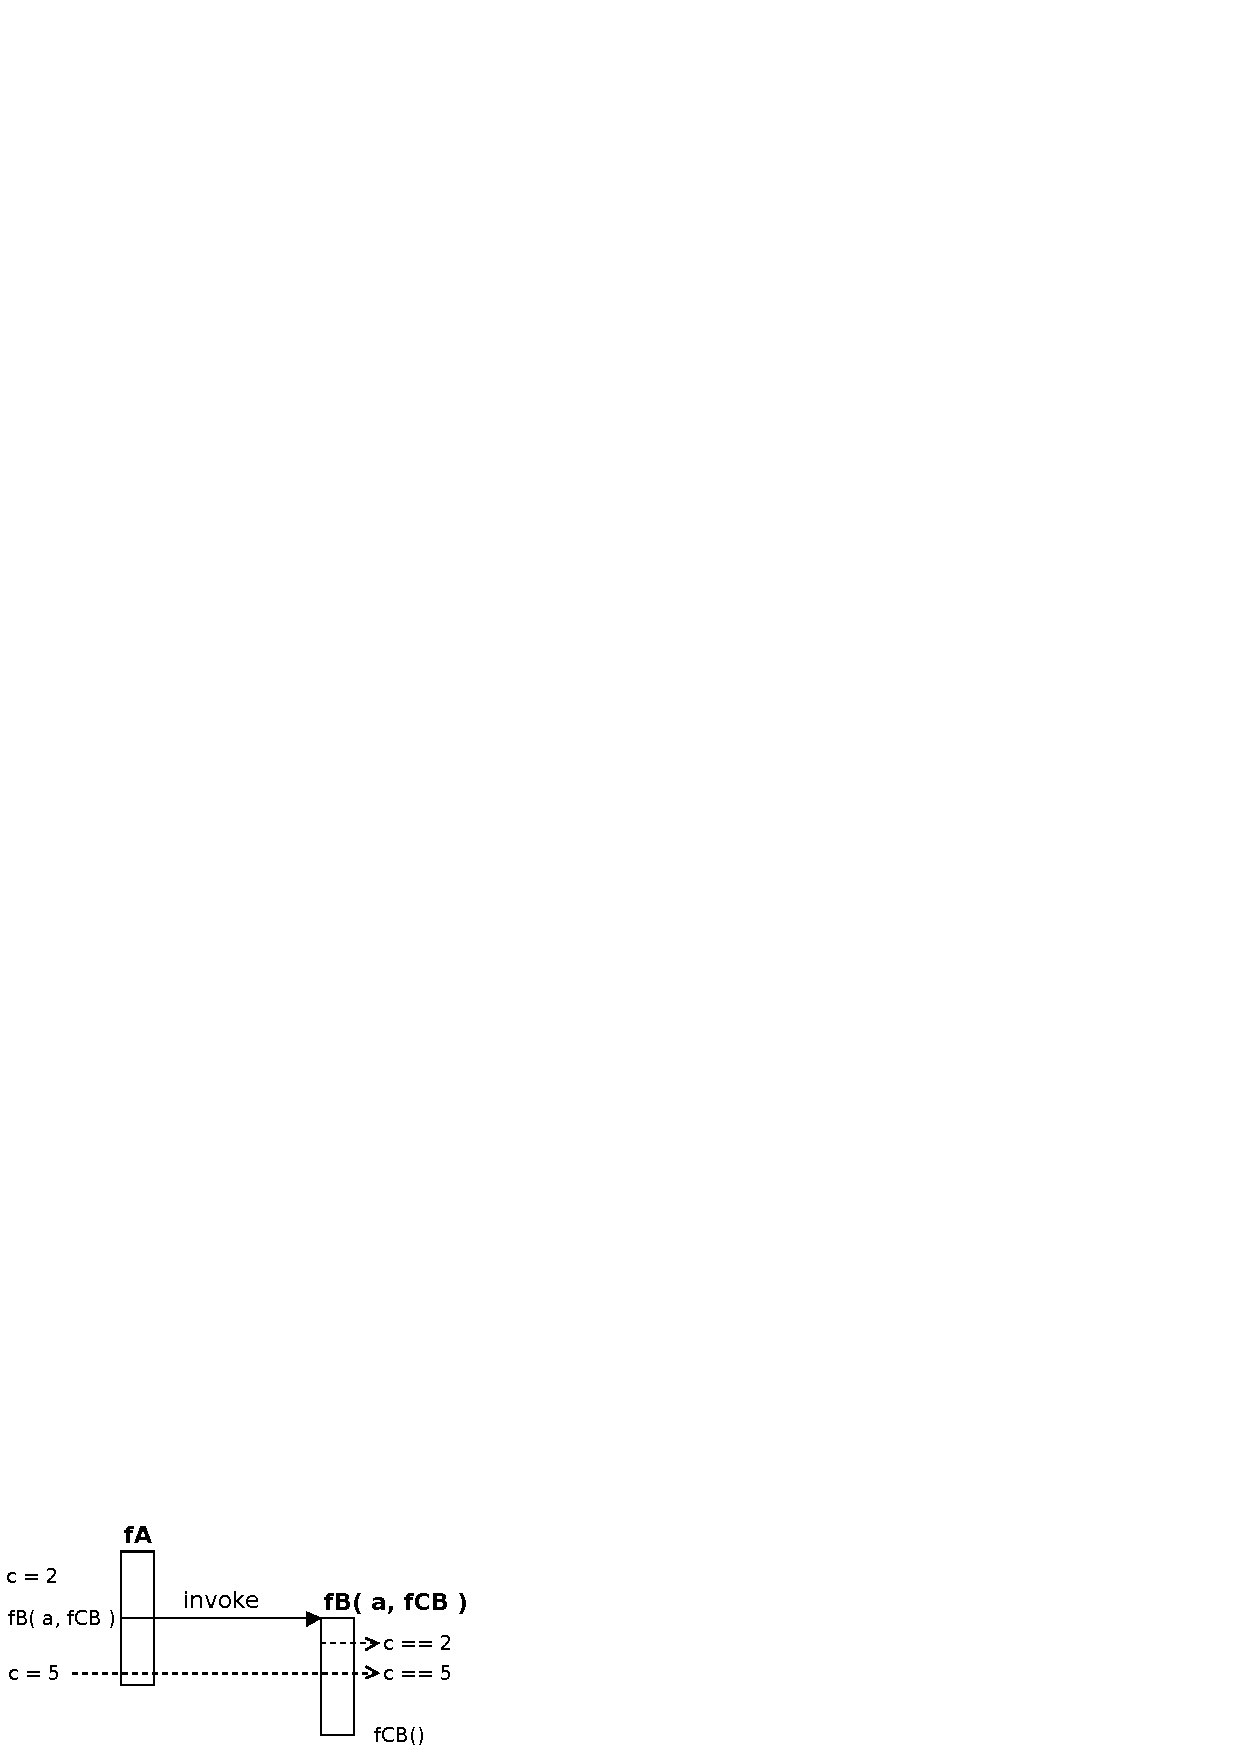
\includegraphics{figures/Closures_Closure-1}}%
\caption{Closure Scope}
%\end{center}
\end{figure*}


\begin{figure*}[htb]
%\begin{center}
\centering
%,angle=-90
  \makebox[\textwidth][c]{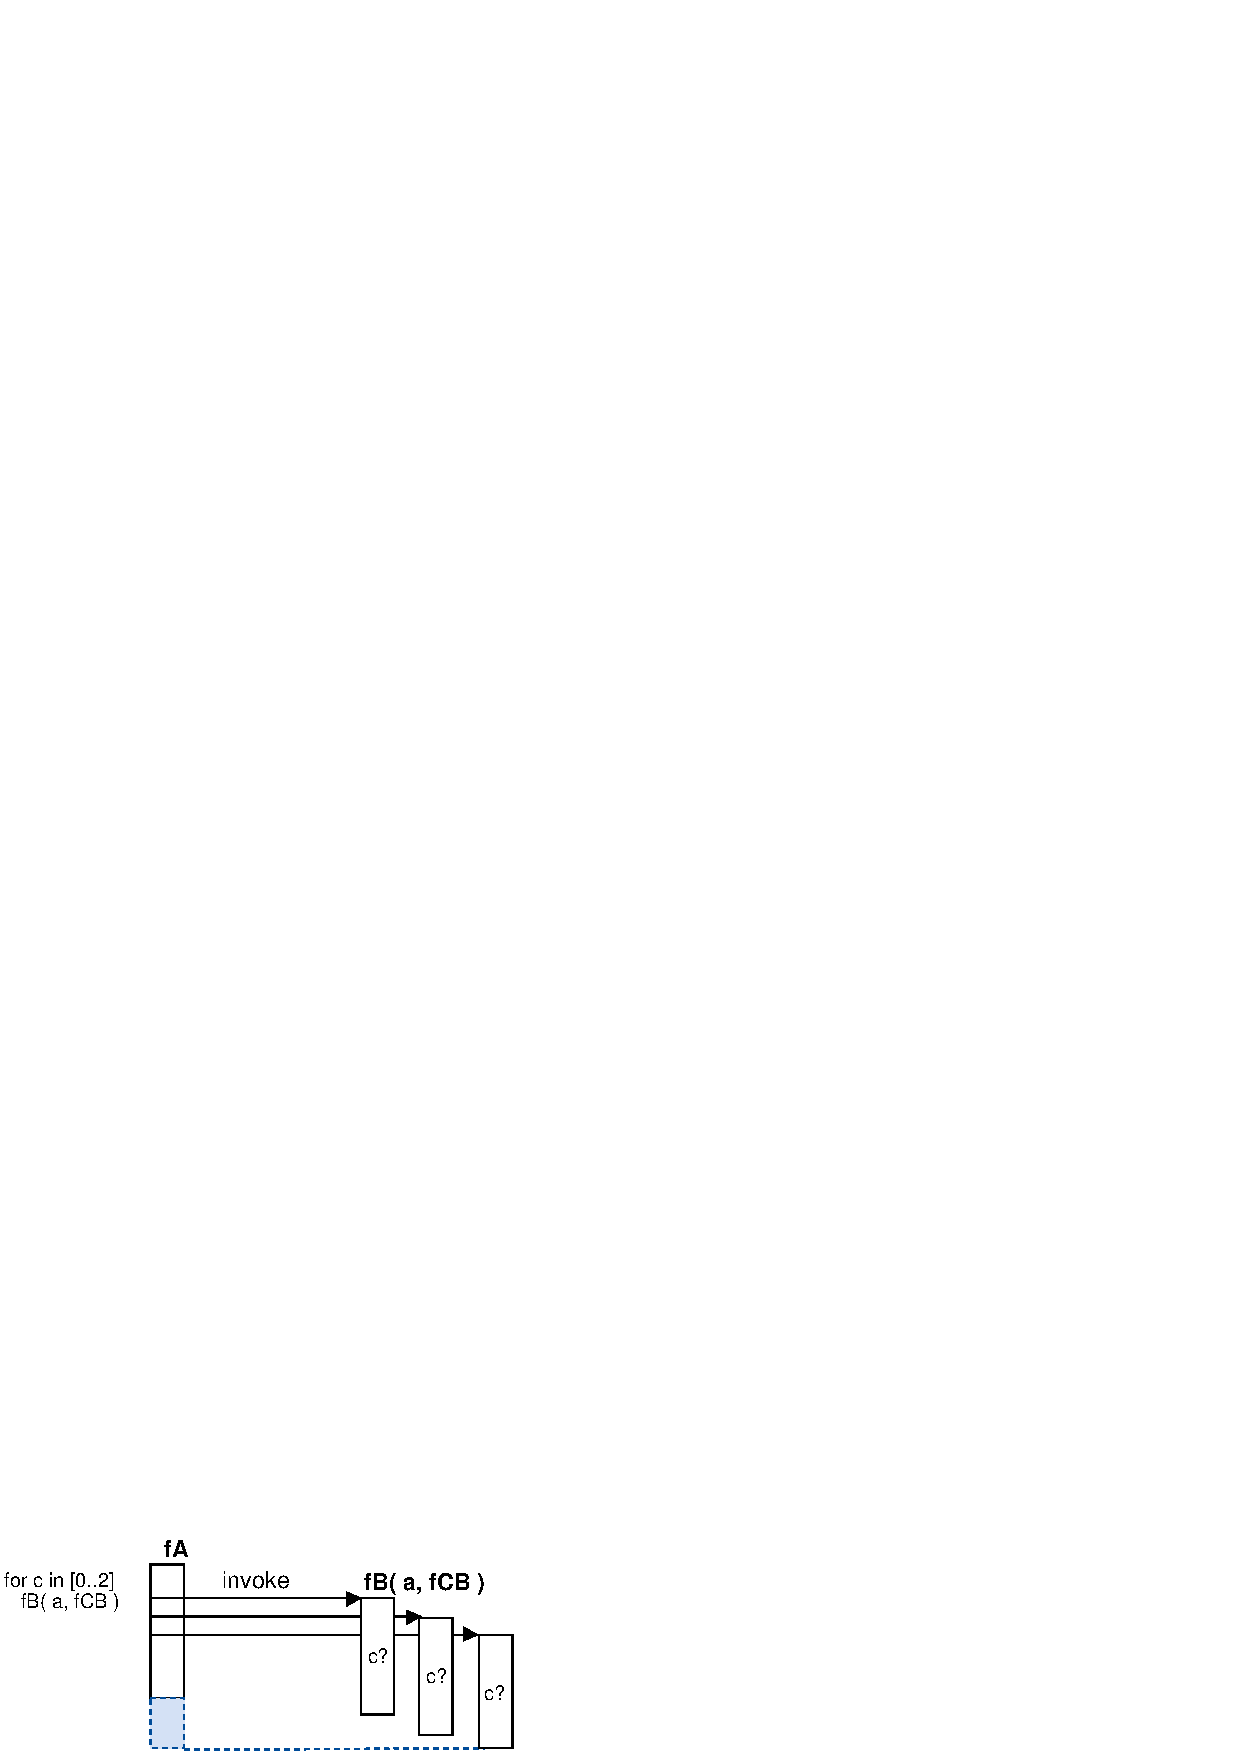
\includegraphics{figures/Closures_Closure-2}}%
\caption{Closure Scope}
%\end{center}
\end{figure*}


\begin{figure*}[htb]
%\begin{center}
\centering
%,angle=-90
  \makebox[\textwidth][c]{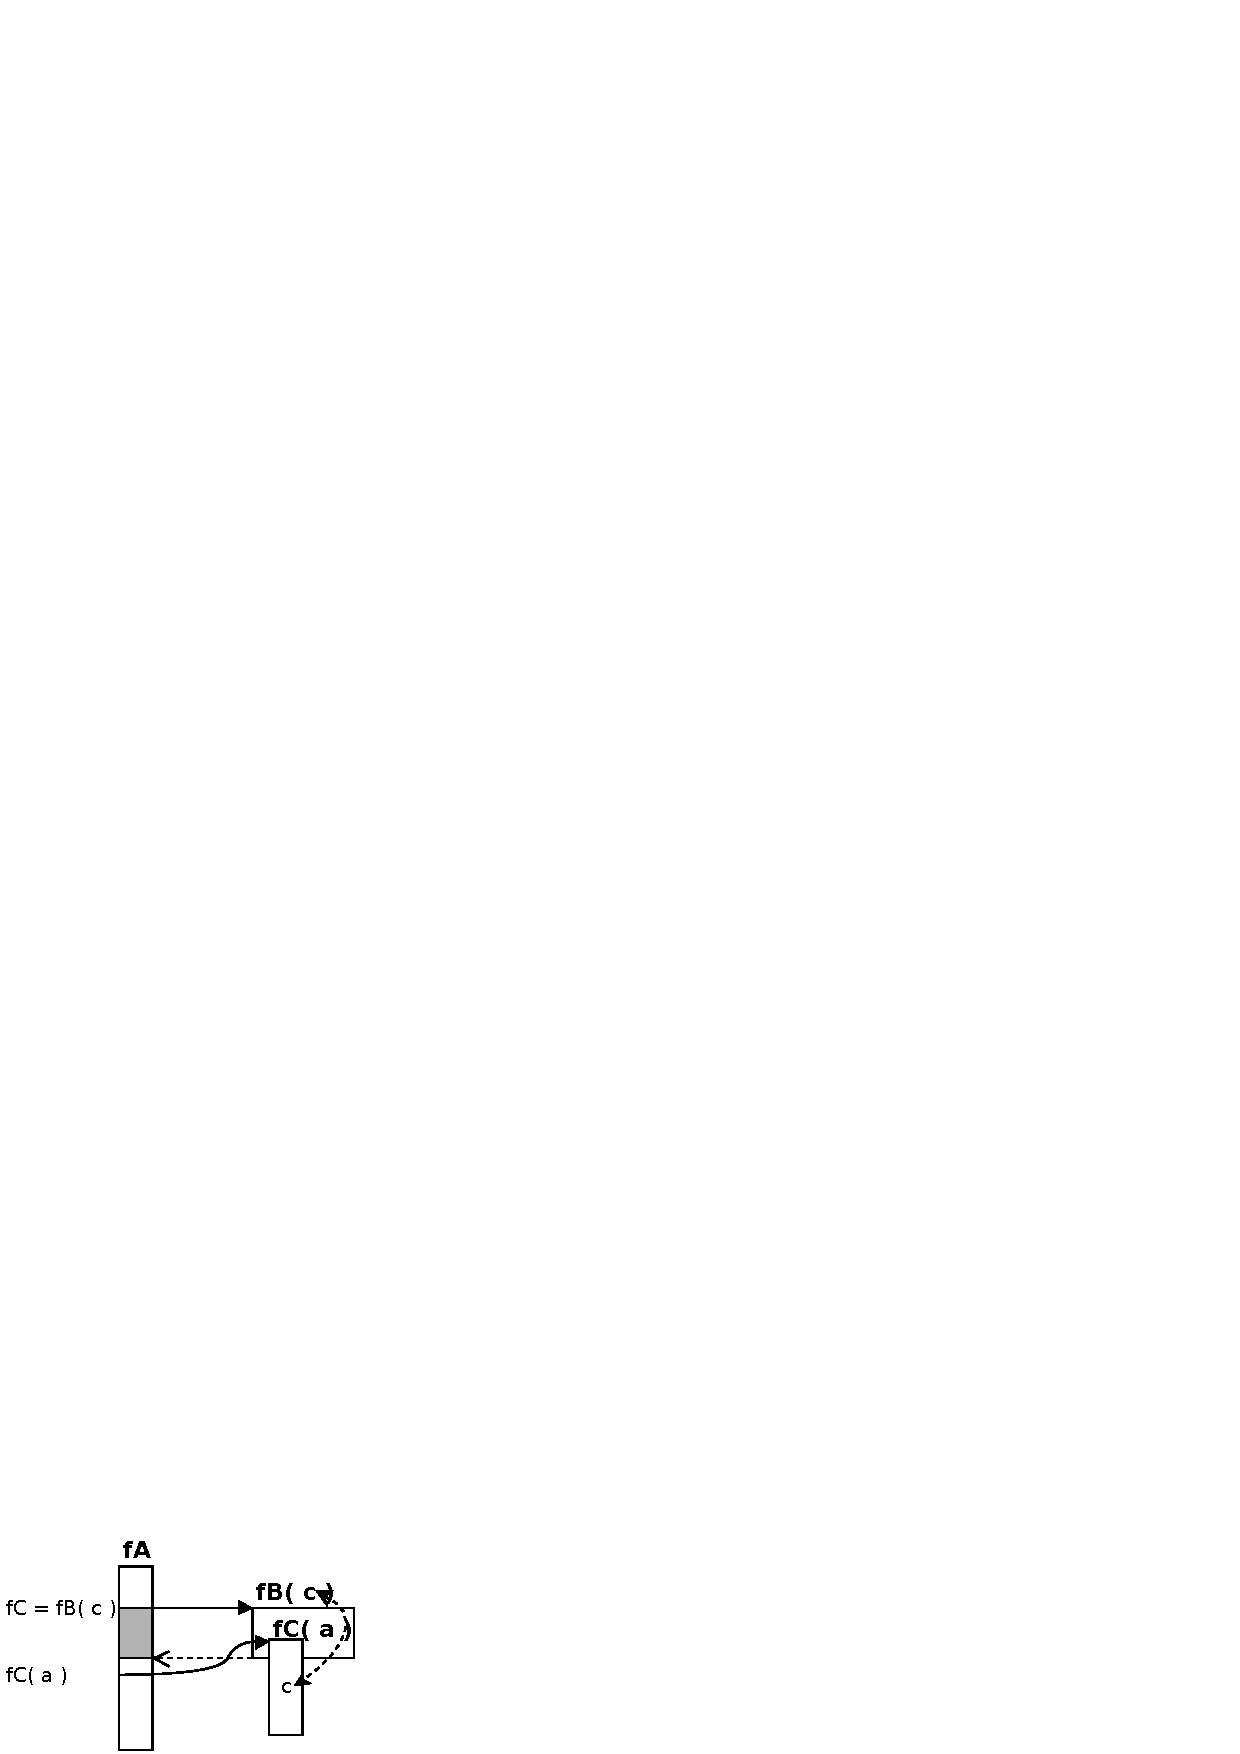
\includegraphics{figures/Closures_Closure-3}}%
\caption{Closure Scope}
%\end{center}
\end{figure*}

% Error tracing
% Apply variable number of function arguments to function
